\chapter{End-to-End Verifiable Voting Using Split-Value Representations} \label{sv}

In this section, we present the split-value system enabling end-to-end verifiable voting as described by Rabin and Rivest \cite{rrv} as well as an overview of the implementation as given in \cite{marco}. We will focus on the main ideas and components of the design and implementation of the system, and leave the explanation of the details to the respective papers.

\section{The Split-Value Voting System Design} \label{sv:design}

\subsection{Definitions} \label{sv:design:defns}

Given an election, choose the \emph{representation modulo} $M$ so that any voter's selection, including possible write-in candidates, may be represented by an integer modulo $M$.

\begin{definition}
The \emph{split-value representation} of $x$ modulo $M$ is the pair $\SV(x)=(u,v)$ such that $x = u+v \bmod M$.
\end{definition}

Note that for a given $x$, knowing the value of one of $u$ or $v$, but not both, reveals no information about $x$. This key property allows us to construct zero-knowledge proofs of equality for two values using their split-value representations, without revealing the actual values themselves.

\begin{definition}
A \emph{commitment} to a value $x$ with randomness $r$ is the value $c = \Com(x, r)$ such that $c$ may be ``opened'' to reveal $x$ and $r$. We desire that the $\Com$ function is both hiding and binding. That is, given $c = \Com(x, r)$, no information is gained about $x$, and it is infeasible to produce another $(x', r')$ such that $c = \Com(x', r')$.
\end{definition}

The HMAC function, with the randomness $r$ as the key, is used as the commitment function in our implementation.

\begin{definition}
Given $\SV(x) = (u, v)$ and randomness $r$ and $s$, the \emph{split-value commitment} of $x$ is $\ComSV(x) = (\Com(u, r), \Com(v, s))$.
\end{definition}

Using split-value commitments, we may construct probabilistic proofs that two values are equal without revealing the value itself. Suppose that a prover wishes to prove that $x = x'$. Given their split value commitments
\begin{align*}
\ComSV(x) &= (\Com(u, r), \Com(v, s)) \\
\ComSV(x') &= (\Com(u', r'), \Com(v', s'))
\end{align*}
the prover claims that there exists a value $t$ such that $t = u - u'$ and $t = v' - v$. This can be true if and only if $x = x'$. With probability $1/2$, the examiner asks for the opening of the ``left'' commitments, in which case the prover gives the values $u$, $r$, $u'$, and $r'$. The verifier checks that the values $\Com(u, r)$ and $\Com(u', r')$ are correct and that $t = u - u'$. With probability $1/2$, the examiner asks for the ``right'' commitments, in which case the prover sends the other components of the split-value commitment. Thus, if $x \neq x'$, a dishonest prover can win with probability at most $1/2$.

\subsection{The Verifiable Mixnet} \label{sv:design:mixnet}

The main component of the split-value system is a verifiable mixnet composed of a $3 \times 3$ grid of mixservers, as shown in Figure \ref{figure:sv:design:mixnet}. These servers are responsible for receiving votes, obfuscating and permuting them, and producing an output list that cannot be traced back to the input list. Denote the mixserver in row $i$ and column $j$ as $P_{i,j}$.

When the voter's vote $w$ is cast on her device (e.g. a tablet), it is broken into three components $x$, $y$, and $z$ such that $w = x+y+z \bmod M$. The device then creates split-value representations of each component. For each component, the split-value representation and its commitment are sent over a secure channel to the first column mixserver of the row corresponding to the component. For example, $x$ and $\ComSV(x)$ are sent to $P_{1,1}$, $y$ and $\ComSV(y)$ are sent to $P_{2,1}$, and so on. Note that because each mixserver only receives one out of three components of the vote, no single server may reconstruct any individual vote (and break voter privacy) without leaked information from at least two other mixservers.

\begin{figure}[t]
\centering
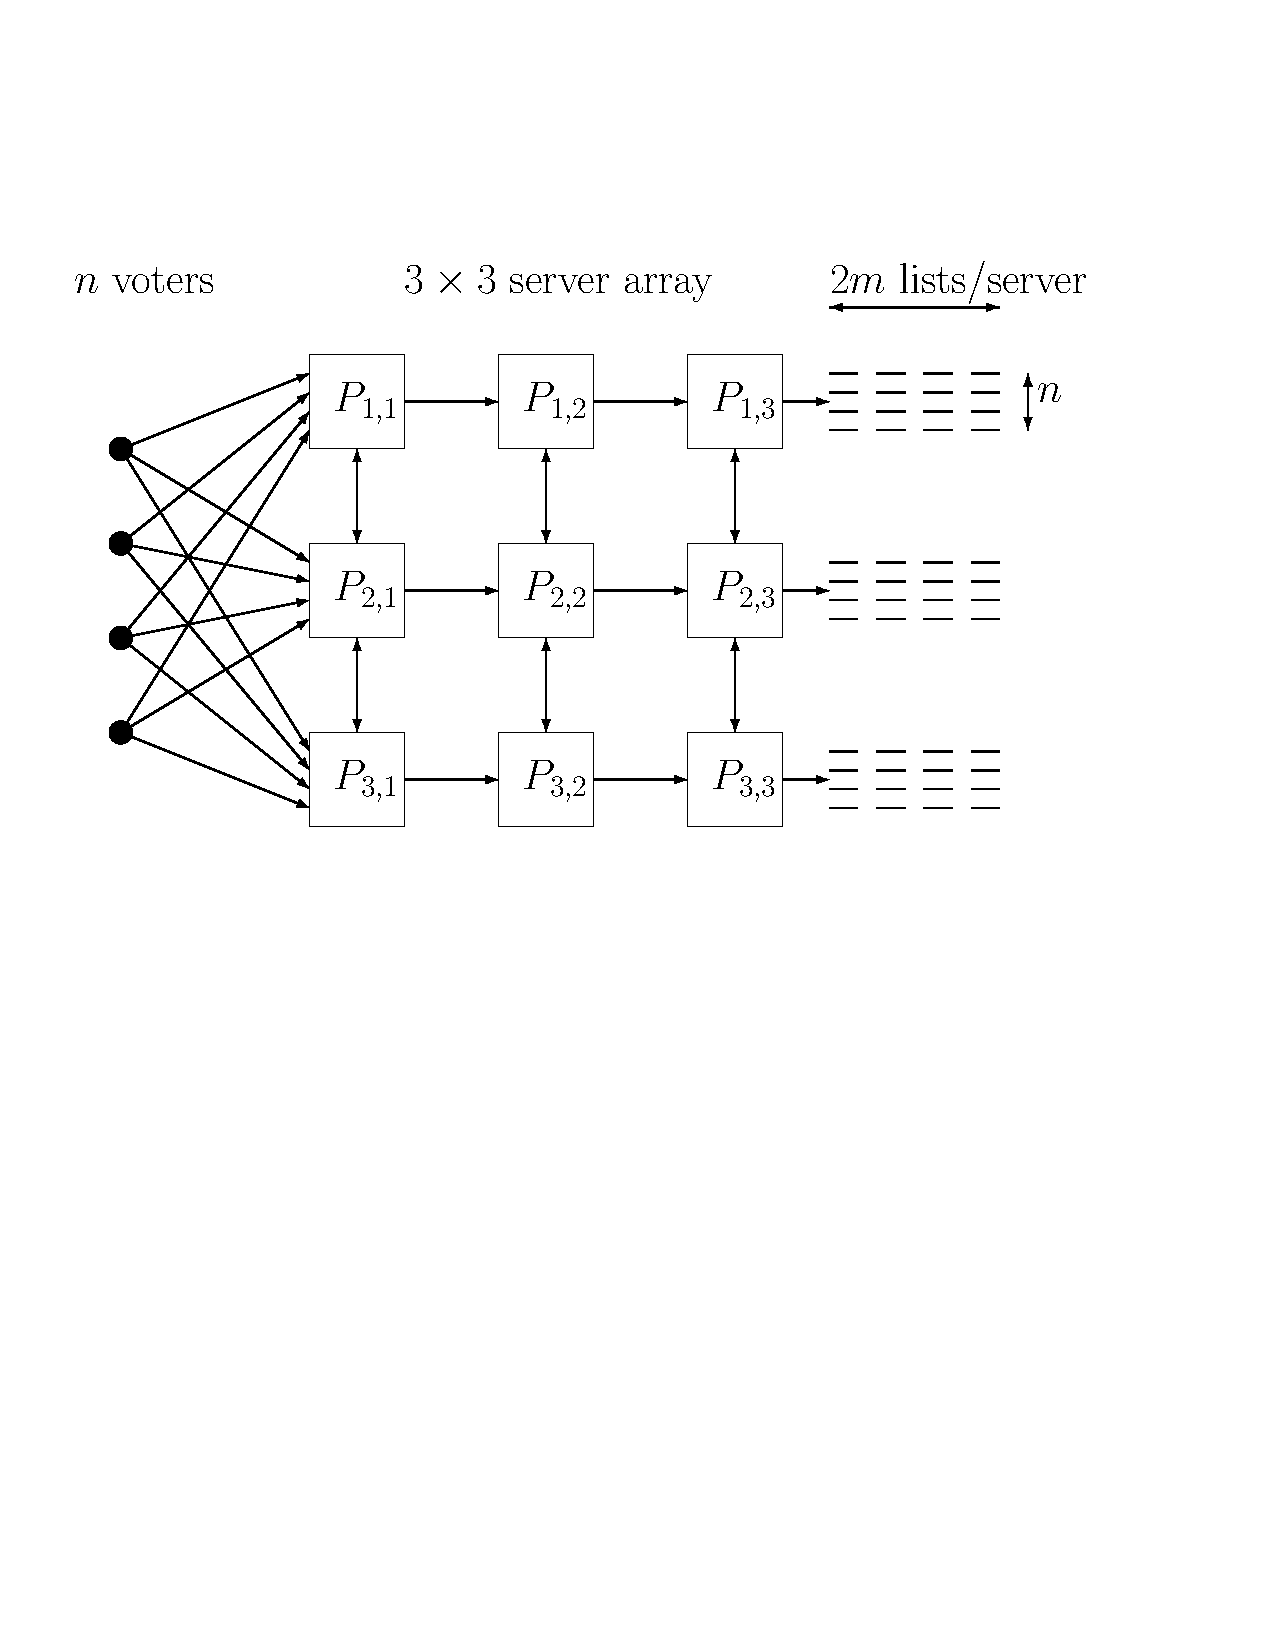
\includegraphics[width=6in]{mixnet-diagram.pdf}
\caption[The $3 \times 3$ grid of mixservers and the communication among them]{The mixnet consists of a $3 \times 3$ grid of mixservers. Votes are split into three components and each component is sent to one of the leftmost servers. Each column of mixservers agree upon a shuffling and obfuscation; the shuffled and obfuscated values are then sent to the next column. The process is repeated $2m$ times.}
\label{figure:sv:design:mixnet}
\end{figure}

\begin{definition}
A triplet $S' = (x', y', z')$ is an \emph{obfuscation} of $S = (x, y, z)$ if $x'+y'+z' = x+y+z \bmod M$.
\end{definition}

The first column of servers agree upon a triplet of values $(p, q, r)$ such that $p + q + r = 0 \bmod M$ for each vote. The first row then computes $x' = x+p \bmod M$, the second row computes $y' = y+q \bmod M$, and so on. The column of servers then agree upon a random permutation $\pi : \{1, \dotsc, n\} \to \{1, \dotsc, n\}$. Each server transmits the permuted obfuscated values to the next column in the same row: $P_{1,1}$ transmits $x'_{\pi(1)}, \dotsc, x'_{\pi(n)}$ to $P_{1,2}$, $P_{2,1}$ transmits the permuted $y'$ values to $P_{2,2}$, and so on.

The second and third columns of mixservers repeat this process, and the results of the final obfuscation and permutation are posted to the secure bulletin board. Given a security parameter $m$, this process of obfuscation and permutation across each column of the mixnet is performed $2m$ times. In our current implementation, $2m = 24$.

To verify the election result, we divide the $2m$ repetitions into two groups of $m$. The first $m$ repetitions are used to show that the mixnet does not alter the votes. To do so, we reveal the permutations used at each column. For each split-value commitment on the input side of the mixnet, we follow the revealed permutations to arrive at its corresponding split-value commitment on the output side and construct a proof of equality as described in the previous section. These permutations and proofs of equality are posted to the secure bulletin board for anyone to examine.

The other $m$ repetitions are used to prove that the election outcome is correct. All of the commitments to the votes are opened, revealing the votes themselves. These votes are posted to the secure bulletin board along with the election outcome for anyone to examine.

\section{Implementation Details} \label{sv:implementation}

The original design of the system included a functioning preliminary prototype written using Python 3.4. In this prototype, mixservers were simulated using Python objects. A simulation of a complete election, including vote generation, mixing, proof construction, and verification, was contained within a single Python process. Python was chosen for its ease of programming, debugging, profiling, and installation. Care was taken to ensure that included libraries was kept to a minimum, so that the code was easy to run and results easily replicated.

\subsection{Server Processes and Communication} \label{sv:implementation:comm}

Subsequent work \cite{marco} significantly decoupled the system. The mixservers, secure bulletin board, and vote generation each became its own process. An interface was built on top of Python TCP socket servers to facilitate communication, and Python socket handlers were used to handle incoming requests. All data was serialized with standard JSON libraries. The implementation also introduced the notion of a \emph{controller server}, whose responsibilities include the following.
\begin{itemize}
\item Serve as the first point of contact for all other servers. All other servers start knowing the IP address and port of the controller.
\item Keep track of and broadcast network information, including all other servers, their addresses, and roles, to the network.
\item Assign roles to each other server, and assign their positions in the mixnet.
\item Synchronize the various phases of the election simulation, including vote production, mixing, proof construction, tallying, and verification.
\end{itemize}

Because all communication occurs via standard TCP sockets, the implementation may be used on any group of computers running on a local area network. The implementation has been tested on single-core and multicore machines as well as multiple virtual machines running on a virtualized network.

\subsection{The Implementation of Randomness} \label{sv:implementation:random}

One particular detail that deserves special attention is the implementation of randomness. Randomness is used throughout the system: in constructing split-value representations, in constructing commitments, in choosing which component of a split-value representation to reveal during a verification, and so on. Fast, cryptographically secure randomness is essential to the correct functioning of the system.

The utility function library written for this implementation includes a function that generates pseudorandom bytes. Each server maintains a list of randomness sources. When a randomness source is created, its name is used as the initial seed. When a sequence of pseudorandom bytes is desired, the seed is hashed twice using the SHA-256 hash function. The first hash determines the updated seed, which is stored in the place of the original seed. The second hash is of the original seed with a ``tweak'' string appended. With a good hash function, these two hashes will not appear to have originated from the same seed.

During the production of the proofs, we require a good source of randomness to choose the $m$ repetitions that will be used to verify the mixnet and the other $m$ repetitions that will be used to verify the election result. There are two options for this.
\begin{itemize}
\item An \emph{external source of randomness}, such as a dice-roll which occurs at a public ceremony after voting has ended. The benefit to this method is that we obtain ``true'' randomness that no adversary can predict beforehand. However, it is possible that election officials and the public are uncomfortable with introducing what appears to be games of chance into the election process.
\item A \emph{Fiat-Shamir style hash} of the secure bulletin board. With overwhelming probability, a Fiat-Shamir style hash of the secure bulletin board will provide randomness that is good enough to overcome an adversary. There is the small but nonzero chance that an adversary could manipulate the election result by providing both a faulty proof that supports the manipulated outcome and an alternate version of the secure bulletin board that, when hashed, produces randomness that verifies her faulty proof. To compensate for this, we set the number of repetitions ($m$) to be higher so that the chance of producing an alternate secure bulletin board that passes all of the verifications decreases exponentially.
\end{itemize}

In the current implementation, we use the Fiat-Shamir method. However, this choice incurs a penalty in performance, as our setting for $m$ could be reduced dramatically by using an external source of randomness, resulting in fewer iterations through the mixnet and a shorter proof. In the next chapter, we will see that the use of an external source of randomness may provide enough of a performance boost to meet certain goals that election officials desire.

\section{Conclusion} \label{sv:conclusion}

In this section, we introduced the concepts and design behind the split-value verifiable voting system, including the idea of a split-value commitment. We discussed the ways that votes are obfuscated and permuted through the mixnet. Proofs are constructed to verify both the mixnet and the election outcome without revealing associating voters with their votes. Finally, we examined details of the prototype implementation, including the communication interface between servers and the implementation of randomness used in our simulations.

